\newpage

\section{可行性分析}

\subsection{重难点分析}

\subsubsection{实现重点}

整车实现的重点主要在于以下几个部分:

\begin{enumerate}
	
	\item 实现平台封装整体体积紧凑,厚度适宜相关机械结构与电子元件的封装,保证整体系统稳定;
	
	\item 实现平台具有有效的悬架避震结构,搭载了刚度可调节的减震器,底盘负载能力大,避免因为云台其他机构的搭载而失去整体系统稳定;
	
	\item 实现平台便于快速开发,适配不同车载机控制器,预留底盘控制程序基础架构,供用户个性化修改,从而快速实现无人驾驶车辆路径跟踪、轨迹控制及动力学控制算法编制;
	
	\item 实现平台预留多种协议的通讯接口及多种电压的供电接口,实现即插即用,满足市面常见激光雷达、毫米波雷达、摄像头、工控机的供电及通讯需求,方便用户进行无人驾驶车辆开发。
	
\end{enumerate}

\subsubsection{待突破难点}

以上重点为AtomIC的核心部分,但是一些部分仍然存在较大难度亟需突破完善:

\begin{enumerate}
	
	\item AtomIC平台目前底盘车身机构未能密闭封装,将有可能限制如泥沼、潮湿等较为恶劣的工况;
	
	\item AtomIC平台所选用的基本款激光雷达较为昂贵,未来将选用恒威稳定可靠但精度尚可的部件作为平台标配;
	
	\item AtomIC平台目前采用四轮双横臂独立悬架系统,主要适用与轻载型应用场景,可对于不同的应用考虑系列化整车平台设计或是可变刚度阻尼的校核与选用。
	
\end{enumerate}

\subsection{经济社会效益分析}

\begin{figure}[htbp]
	\centering
	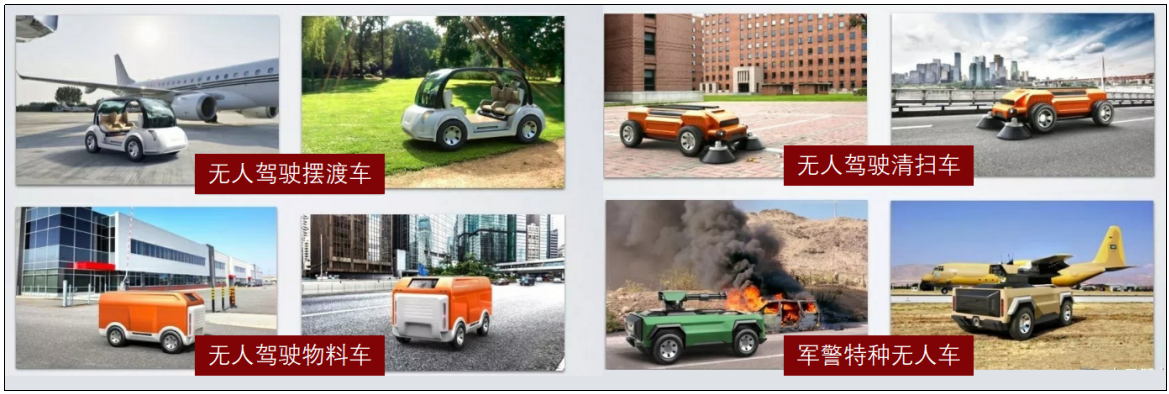
\includegraphics[width = 0.8\textwidth]{fig/wlknyy.png}
	\caption{未来可能应用}
	\label{wlknyy}
\end{figure}

未来以AGV小车和无人驾驶技术为主要核心的特定场景应用将可能会全面铺开,在图\ref{wlknyy}中我们可以看到目前已经正在发展的集中解决“痛点”的应用

然而目前自动驾驶小车采用低成本的电动代步车底盘改装成为了现行主要解决方案,但其行驶速度、机动能力、载重能力和平顺性等较差。同时,电动代步车底盘本身是面向有人驾驶的,其存在着诸多问题,如转向盘等机械结构冗余、线控化程度低、续航能力差、电池系统不满足车规级需求、控制系统粗糙、执行元件精度低等,难以满足无人驾驶车辆实际的性能需求。更重要的是,当前用于改装的底盘五花八门、改装方案良莠不齐,因此我认为AtomIC平台的推出将会有利于促进未来特定场景无人驾驶车辆的算法实验测试与实际联网等场景的高效运作,主要技术有点如下:

\begin{enumerate}
	
	\item AtomIC平台封装体积极小,厚度小于30cm,将可方便用户进行个性化上装车壳造型订制。
	
	\item AtomIC平台封装集成高能量密度锂动力电池、电池管理系统、四轮电机转向系统、底盘快速开发控制器及CAN网络通讯系统。控制系统及执行元件达到车规级需求,响应速度快、反馈精度高。
	
	\item AtomIC平台采用基于Simulink环境的车规级底盘快速开发控制器,预留底盘控制程序基础架构,供用户个性化修改,从而快速实现无人驾驶车辆路径跟踪、轨迹控制及动力学控制算法编制。
	
	\item AtomIC平台封装车身上预留了多种协议的通讯接口,及多种电压的供电接口,实现即插即用,满足市面常见激光雷达、毫米波雷达、摄像头、工控机的供电及通讯需求,方便用户进行无人驾驶车辆开发。
	
	\item AtomIC平台采用四轮双横臂独立悬架系统,并搭载了刚度可调节的减震器,底盘负载能力大。
	
\end{enumerate}

未来希望能够有这样一款高效、快速以及性能优良的产品出现,将会大大有利于中国在二三产业的发展,实现“中国制造2025”的落地。